% energy.tex
% $Author$ $Date$

% Predrag                   Apr 12 2007

\subsection{Energy budget} % of the \KSe}
\label{sec:energy}

In physical settings where the observation times are much longer
than the dynamical ``turnover" and Lyapunov times (statistical mechanics,
quantum physics, turbulence) nonlinear dynamics provides 
\cite{DasBuch} highly accurate predictions of measurable
long-time averages such as the turbulent drag\cite{GHCW07}.

Physical predictions have to be independent of the choice of
basis in which the PDE is represented as an infinite tower of
ODEs - and - most importanly - of any symmetry of the problem.
In this section we discuss and compute
a set of such physical observables for
the  1$D$ KS invariant under reflections and translations.

The {space average} of a function $\obser = \obser(\pSpace,t)$  on
the interval $L$,
\beq
    \expct{\obser} = \Lint{\pSpace}\, \obser(\pSpace,t)
    % \expct{\obser} = \frac{1}{L}\int_0^{L} d\pSpace\, \obser(\pSpace,t)
    \,,
    \label{rpo:spac_ave}
\eeq
is in general time dependent. 
Its mean value is given by the {time average}
\beq
\timeAver{\obser}
    =
\lim_{t\rightarrow \infty} {1\over t} \int_0^t \! d\tau \, \expct{\obser}
    =
\lim_{t\rightarrow \infty} {1\over t L} \int_0^t \! 
    \int_0^{L} \!\! d\tau  d\pSpace\, \obser(\pSpace,\tau)
    \,.
\label{rpo:tim_ave}
\eeq
The mean value
$\timeAver{\obser}$, $\obser = \obser(u)$ evaluated on an
\eqv\ or {\reqv} $u(\pSpace,t) = u_q(\pSpace-ct)$ is
\beq
         \obser_q = \expct{\obser}_q
\,.
\label{rpo:u-eqv}
\eeq
Evaluation of the infinite time average \refeq{rpo:tim_ave}
on a function of a period $\period{p}$
\po\ or \rpo\ $u_p(\pSpace,t)$
 requires only a single traversal of the periodic solution,
\beq
       \obser_p = \frac{1}{\period{p}}
    \int_0^{\period{p}} \! d\tau \, \expct{\obser}
\,.
\label{rpo:u-cyc}
\eeq

Equation \refeq{ks} can be written as % in ``potential'' form
\beq
    u_t=- V_x
        \,,\qquad
    V(x,t)={\textstyle\frac{1}{2}}u^2+u_{x} + u_{xxx}
    \,.
\ee{ksPotent}
$u$ is related to the ``flame-front height'' $h(x,t)$ by
$u=h_x$, so \expctE\ can be interpreted as
the mean energy density \refeq{ksEnergy}.
%
So, even though KS is a phenomenological
small-amplitude equation, the time-dependent quantity
\beq
    \expctE=\frac{1}{L}\int_0^{L} \!dx \, V(x,t)
    =\frac{1}{L}\int_0^{L}\! dx \, \frac{u^2}{2}
\label{ksEnergy}
\eeq
% \PC{this is missing a prefactor 1/2. Check if someone in literature
% - other than Greene and Kim - defines it right. }
has a physical interpretation\rf{ksgreene88}
as the average ``energy'' density of the flame front.
This analogy to the corresponding definition of the
mean kinetic energy density for
the Navier-Stokes will be useful in what follows.
\PC{bit weird: can use Galilean invariance to
    set $\expctE=0$ for any given $u(x,t)$?}

The energy \refeq{ksEnergy} is intrinsic to
the flow, independent of the particular ODE basis set 
chosen to represent the PDE. However, as the Fourier
amplitudes are eigenvectors of the translation operator,
in the Fourier space the energy is a diagonalized
quadratic norm,
\beq
\expctE   % = (u,u) 
          = \sum_{k=1}^{\infty} E_k
\,,\qquad
E_k = % a_{-k} a_k =
    {\textstyle\frac{1}{2}}|a_k|^2
\,,
\ee{EFourier}
and explicitely invariant term by term 
under translations \refeq{eq:RPO}.

Take time derivative of the energy density \refeq{ksEnergy},
substitute \refeq{ks} and integrate by parts. Total derivatives vanish
by the spatial periodicity on the $L$ domain:
\bea
   \dot{\expctE} &=&
     \expct{u_t \, u}
    % \frac{1}{L}\int_0^{L}u \, u_t\, dx
     = - \expct{\left(\frac{u^2}{2} + u \, u_{x} + u \, u_{xxx}\right)_x u }
    \continue
    &=&
\expct{+ u_x \, \frac{u^2}{2} + (u_{x})^2 + u_x \, u_{xxx}}
    \,.
\label{rpo:ksErate}
\eea
Substitution by \refeq{KSeqvCond}
verifies that for an \eqv\ $\expctE$ is constant:
\[
   \dot{\expctE} =
\expct{ \left(\frac{u^2}{2} + u_{x} + u_{xxx} \right) u_x}
    = \expctE \expct{ u_x }=0
    \,.
\]
The first term in \refeq{rpo:ksErate} vanishes by
integration by parts,
\(
 \expct{(u^3)_x} = 3 \expct{ u_x \, u^2}=0
\,,
\) % {EnNonl0}
and integrating the third term by parts yet again we get
that the energy variation
% \PC{this is ``power", nicht war?}
\beq
   \dot{\expctE} = P - D
		\,,\qquad
      P =  \expct{(u_{x})^2}
		\,,\quad
      D =  \expct{(u_{xx})^2}
\ee{EnRate}
balances the KS equation \refeq{ks} power $P$
pumped in by the anti-diffusion $u_{xx}$
against energy dissipation rate $D$
by the hypervicosity $u_{xxxx}$ \rf{ksgreene88}.

%%%%%%%%%%%%%%%%%%%%%%%%%%%%%%%%%%%%%%%%%%%%%%%%%%%%%%%%%%%%%%%%
\begin{figure}[t] 
\begin{center}
    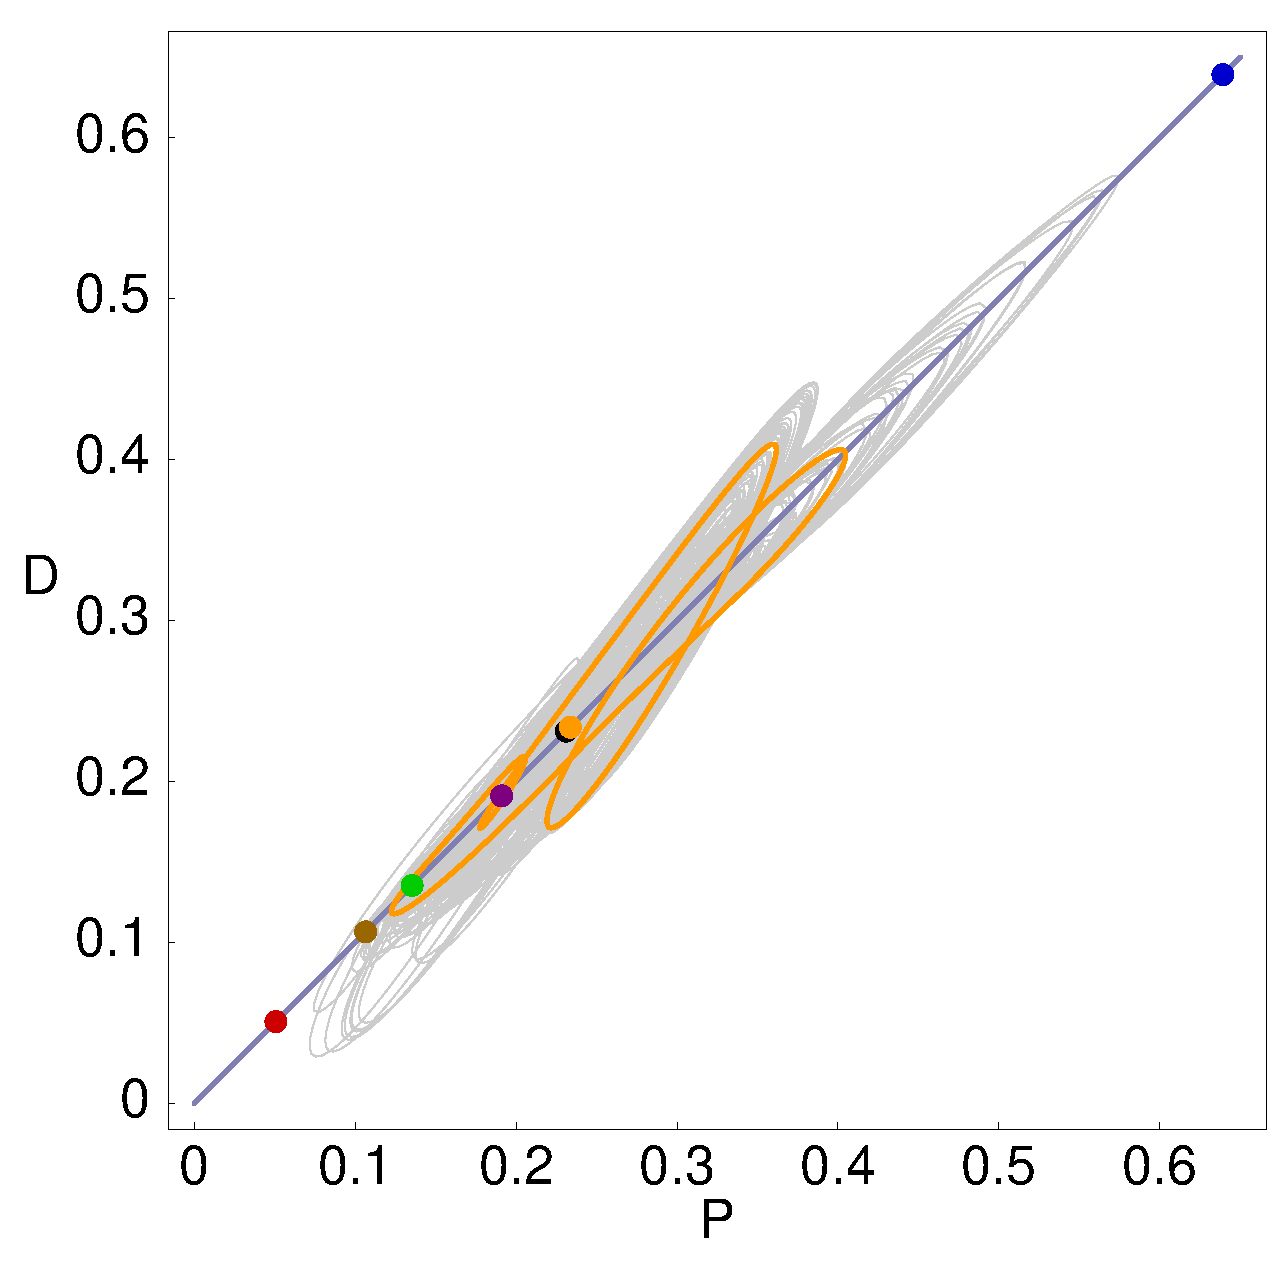
\includegraphics[width=0.8\textwidth]{figs/energyBalancePlot.eps}
\end{center}
\caption{
Power input $P$ vs.
dissipation rate $D$ for $L=22$ \eqva\
and \reqva, for several
% \ESedit{(two, more in the way!)}
\po s and \rpo s, and for a typical ``turbulent"
state.
\label{f:drivedrag}
\end{figure}
%%%%%%%%%%%%%%%%%%%%%%%%%%%%%%%%%%%%%%%%%%%%%%%%%%%%%%%%%%%%%%%%%%

%%%%%%%%%%%%%%%%%%%%%%%%%%%%%%%%%%%%%%%%%%%%%%%%%%%%%%%%%%%%%%%%
\begin{figure}[t] 
\begin{center}
    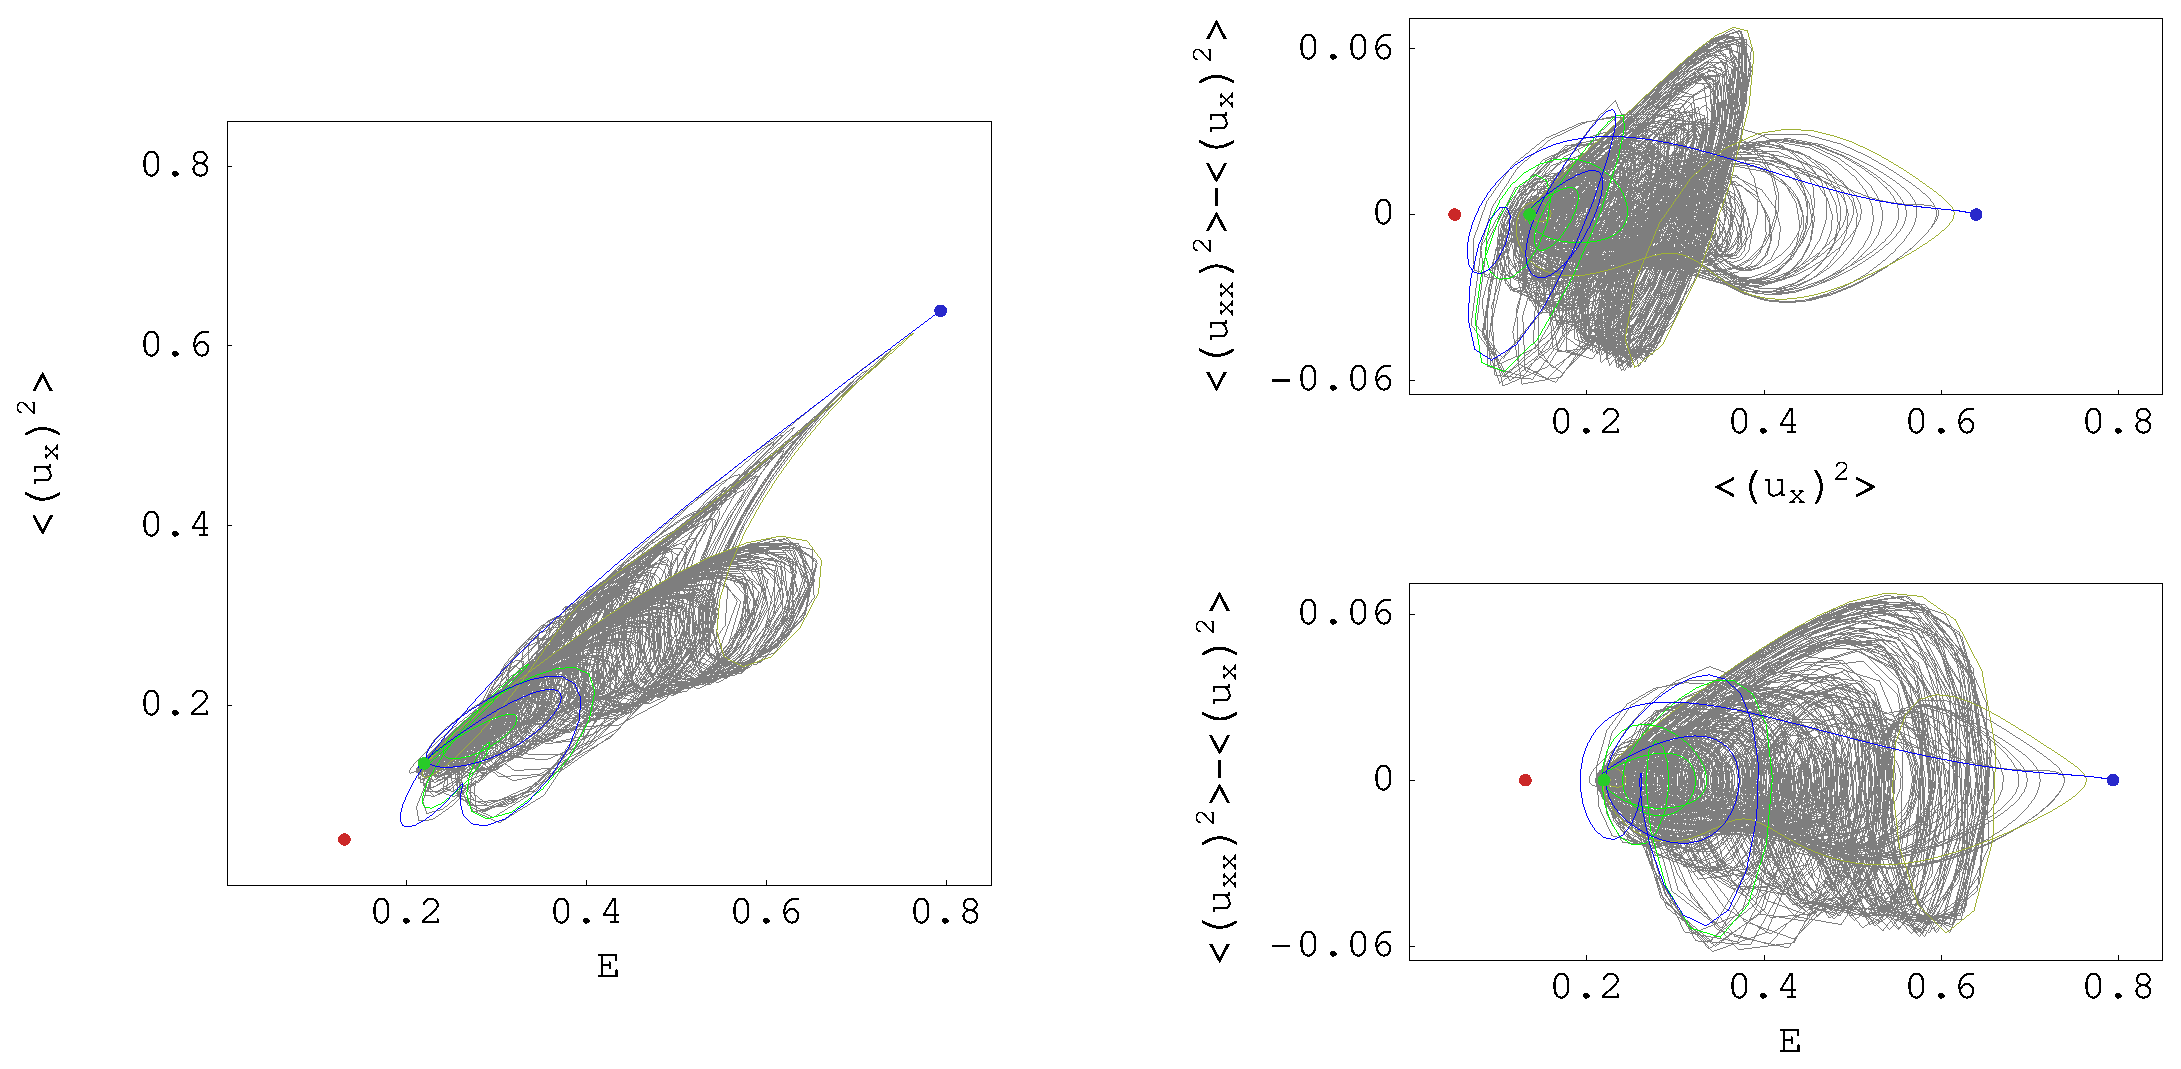
\includegraphics[width=0.8\textwidth]{figs/ks22TurbConn_xfig.eps}
\end{center}
\caption{
\EQV{1} (red), \EQV{2} (green), \EQV{3} (blue), 
connections from \EQV{1} to $A(L/4)\EQV{1}$ (green),
from $A(L/4)\EQV{1}$ to \EQV{1} (yellow-green) 
and from \EQV{3} to $A(L/4)\EQV{1}$ (blue), along
with a generic long-time ``turbulent" evolution (grey) for $L=22$. 
Three different projections of the 
$(E,P,D-P)$
representation.
        }
\label{f:drivedragConn}
\end{figure}
%%%%%%%%%%%%%%%%%%%%%%%%%%%%%%%%%%%%%%%%%%%%%%%%%%%%%%%%%%%%%%%%%%

\PC{
 Implementing Ruslan: all axes in \reffig{f:drivedragConn} changed by a factor
of 4?
	\\
Implementing Predrag: 
label axes in \reffig{f:drivedrag}, \reffig{f:drivedragConn}
by $(E,P,D)$
    }
\PC{ks22TurbConn2\_xfig.eps for \reffig{f:drivedragConn}
    not checked in?
   }
In \reffig{f:drivedrag}
we plot the power input $P$ {\em vs.} %$\expct{(u_{x})^2}$ vs.
dissipation rate $D$ %$\expct{(u_{xx})^2}$
for all $L=22$ \eqva\ and
\reqva\ \PCedit{determined so far},
several \po s and \rpo s, and for a typical ``turbulent"
evolution.
% Notice that the single \rpo\ with $T\simeq32$ captures a large
% part of the turbulent dynamics
% \ES{Momentarilly adopting Japanese philosophy,
% before putting there the rest of the short orbits.}.
\PC{Re \reffig{f:drivedrag}:
%    (0) replace $y$-axis by
%    $\expct{(u_{xx})^2}-\expct{(u_{x})^2}$, so all \po s lie
%    on the $x$-axis and on can see more clearly the turbulent and
%    periodic trajectory, instead having them scrunched into the
%    diagonal. (a) Replace by side views of
%    3-$d$ $(\expct{u^2},\expct{(u_{x})^2},\expct{(u_{xx})^2}
%       -\expct{(u_{x})^2})$,
%    two figures; 
    (b) current type figure, with chaotic trajectory,
    all \eqva, $(32.\cdots,11)$ as example of well embedded, and
    a typical \po\ {\em not} embedded into the ``turbulent" attractor.
    (c) a separate figure with more \po s, no ``turbulent" attractor.
%    (d) prepare a mathematica macro that automatically uses
%    fonts at least twice the size you use currently. 
    (e) replace
    gray window with a white background, black font. (f) in the
    publication version replace colored dots with symbols of varying
    shapes, fine black border, can be filled in with colors.
    }
%\PC{In \reffig{f:drivedrag}:
%    do also try plotting the heteroclinic connections - they are
%    presumably off the diagonal
%   }
\PC{believe it or not, we are now set to compute
    $\timeAver{E}$ and $\timeAver{P}$
    using cycle expansions
    }
The time averaged energy density  $\timeAver{E}$
computed on a typical orbit goes to a constant, so
the expectation values \refeq{rpo:EtimAve} of drive and dissipation
exactly balance each out:
\beq
    \timeAver{\dot{E}}  =
    \lim_{t\rightarrow \infty}
        {1\over t} \int_0^t d\tau \, \dot{\expctE}
=
      \timeAver{P} - \timeAver{D}
%       \timeAver{(u_{x})^2} - \timeAver{(u_{xx})^2}
= 0
    \,.
\ee{rpo:EtimAve}
In particular, the \eqva\
and \reqva\ sit on the diagonal in \reffig{f:drivedrag},
and so do time averages computed on \po s and \rpo s:
\beq
\timeAver{E}_p =
{1\over \period{p}} \int_0^\period{p}d\tau \, E(\tau)
    \,,\qquad
\timeAver{P}_p =
{1\over \period{p}} \int_0^\period{p} d\tau \, P(\tau)
    =
      \timeAver{D}_p
% \timeAver{(u_{x})^2}_p =
% {1\over \period{p}} \int_0^\period{p} d\tau \, \expct{(u_{x})^2}
%     =
%       \timeAver{(u_{xx})^2}_p
    \,.
\label{poE}
\eeq

In the Fourier basis \refeq{EFourier} the conservation of energy on average
takes form
\beq
0 = \sum_{k=1}^{+\infty} ( (k/\tildeL)^2 - ( k/\tildeL)^4 )\,
    \timeAver{E_k}
\,,\qquad
E_k(t) =  |a_k(t)|^2
\,.
\ee{EFourier1}
The large $k$ convergence of this series is insensitive to the
system size $L$; $\timeAver{E_k}$ have to decrease much faster than
$1/( k/\tildeL)^4$.
\PC{determine the decay rate, presumably exponential in $k$}
Deviation of $E_k$ from this bound for small $k$ determines the active modes.
This may be useful to bound the number of equilibria, with
the upper bound given by zeros of a small number
of long wavelength modes.
For \eqva\ the $L$-independent bound
    on $E$ is given by Michaelson\rf{Mks86}. 
The best current bound\cite{GiacoOtto05,bronski-2005} on the long-time limit
of $E$
as a function of the system size $L$ scales as 
$E \propto L^{3/2}$.
%
\PC{
 % Past: Michael Loss has not taught us how to bound $E$ by
 %  Sobolev bounds. Neither has Spiegel. Next: But 
  Constantin says that the answer is in
    \refrefs{temam85ks}. Eckmann says: the  best bound is by Otto\cite{GiacoOtto05}; the
    only bound close to k=0, better in essential way. See also \refref{bronski-2005}.
    Eckmann had $L^{8/5}$, but conceptually Otto is the best. Recheck whether it is
    $|u|$ or $E \propto L^{3/2}$.
    When the solution is big, how long can it stay big? They found it cannot stay big for
    long. 
       }
\PC{
from bounds on energy, we might be able
to bound the number of equilibria as function of systems size $L$, and thus
be sure we have them all.
   }
%
\PC{Next for fluid guys: read Lieb and Ruelle to learn
    how to bound $E$ for plane Couette by Sobolev bounds}

    \PublicPrivate{%
        }{% switch to Private:
Worked out with Bridges a number of other identities for moments of
\reqv\ $u$, such as
\[
\expct{u_{x} u_t} 
    \qquad \to \qquad
c= \expct{u(u_{x})^2}/P % \expct{(u_{x})^2}
\]
\[
\expct{u_{xx} u_t} 
    \qquad \to \qquad
0= - \expct{(u_{x})^3}/2  + P - \expct{(u_{xxx})^2}
\]
    } %end \PublicPrivate{%

Projections 
\reffigs{f:drivedrag}{f:drivedragConn}
from $\infty$-dimensional \statesp\ to 3-dimensional
$(E,P,D)$ representation of the flow can be a bit misleading
For example, the mean value of $\timeAver{P_p}$
evaluated on the
$(\period{p},\shift_p) =(32.8,10.96)$
 {\rpo}, \reffig{f:ks22rposShort}(c), which appears well embedded
within the turbulent state, is quite close to the turbulent
expectation $\timeAver{P}$.
Similarly close prediction of mean dissipation rate in the
\pCf\ from a single-period \po\ computed by
Kawahara and Kida~\cite{KawKida01} has lead to 
optimistic hopes that ``turbulence" is different from
low-dimensional chaos, and that one \po\ suffices for long-time
predicitions. Regrettably, not true - here too one needs a hierarchy
of \po s of increasing length to obtain accurate
predictions \cite{DasBuch}.
\PC{\PCedit{ the Japanese heresy disposed off}}

The most one can say is that if points are clearly separated in an
$(E,P,D)$ plot (for example, in \reffig{f:ks22rposShort}
$\EQV{1}$ is not part of the recurrent set), they are also separated
in the full \statesp. Converse is not true - states of 
very different topology can have similar energies.
